\noindent
Cuando proyectamos un escena del mundo real en tres dimensiones a un plano de dos dimensiones como la película o el sensor de una cámara, se produce una transformación en la imagen.
Esta transformación, que se conoce como transformación proyectiva, provoca que las líneas paralelas en el mundo real al proyectarse en el plano de la cámara se intersecten en un punto. A dicho punto se le conoce como punto de fuga.

\begin{figure}[!ht]
    \centering
    \begin{subfigure}{0.4\textwidth}
        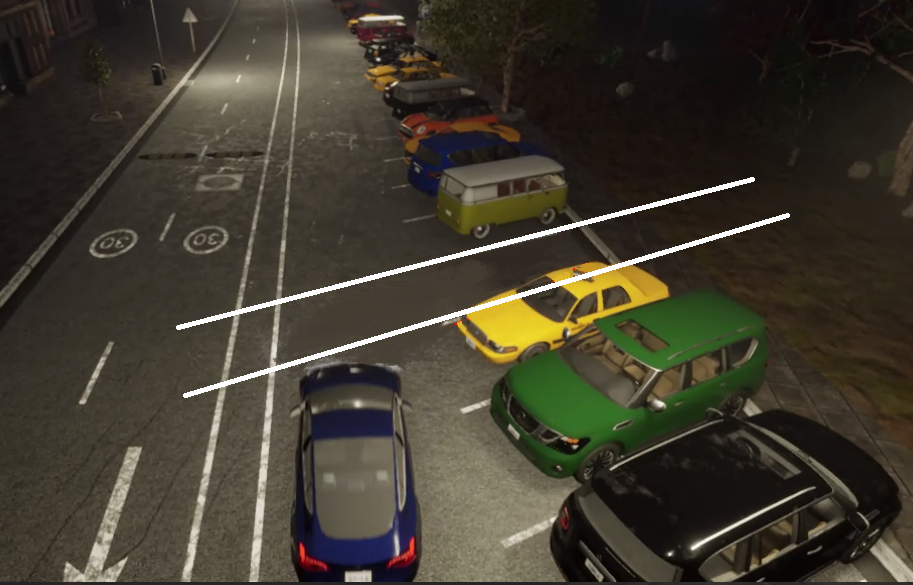
\includegraphics[width=\textwidth]{img/reticule/paralel_lines}\label {fig:parallel_lines}
        \caption{Ejemplo de líneas paralelas en un escenario real en 3 dimensiones}
    \end{subfigure}
    \begin{subfigure}{0.4\textwidth}
        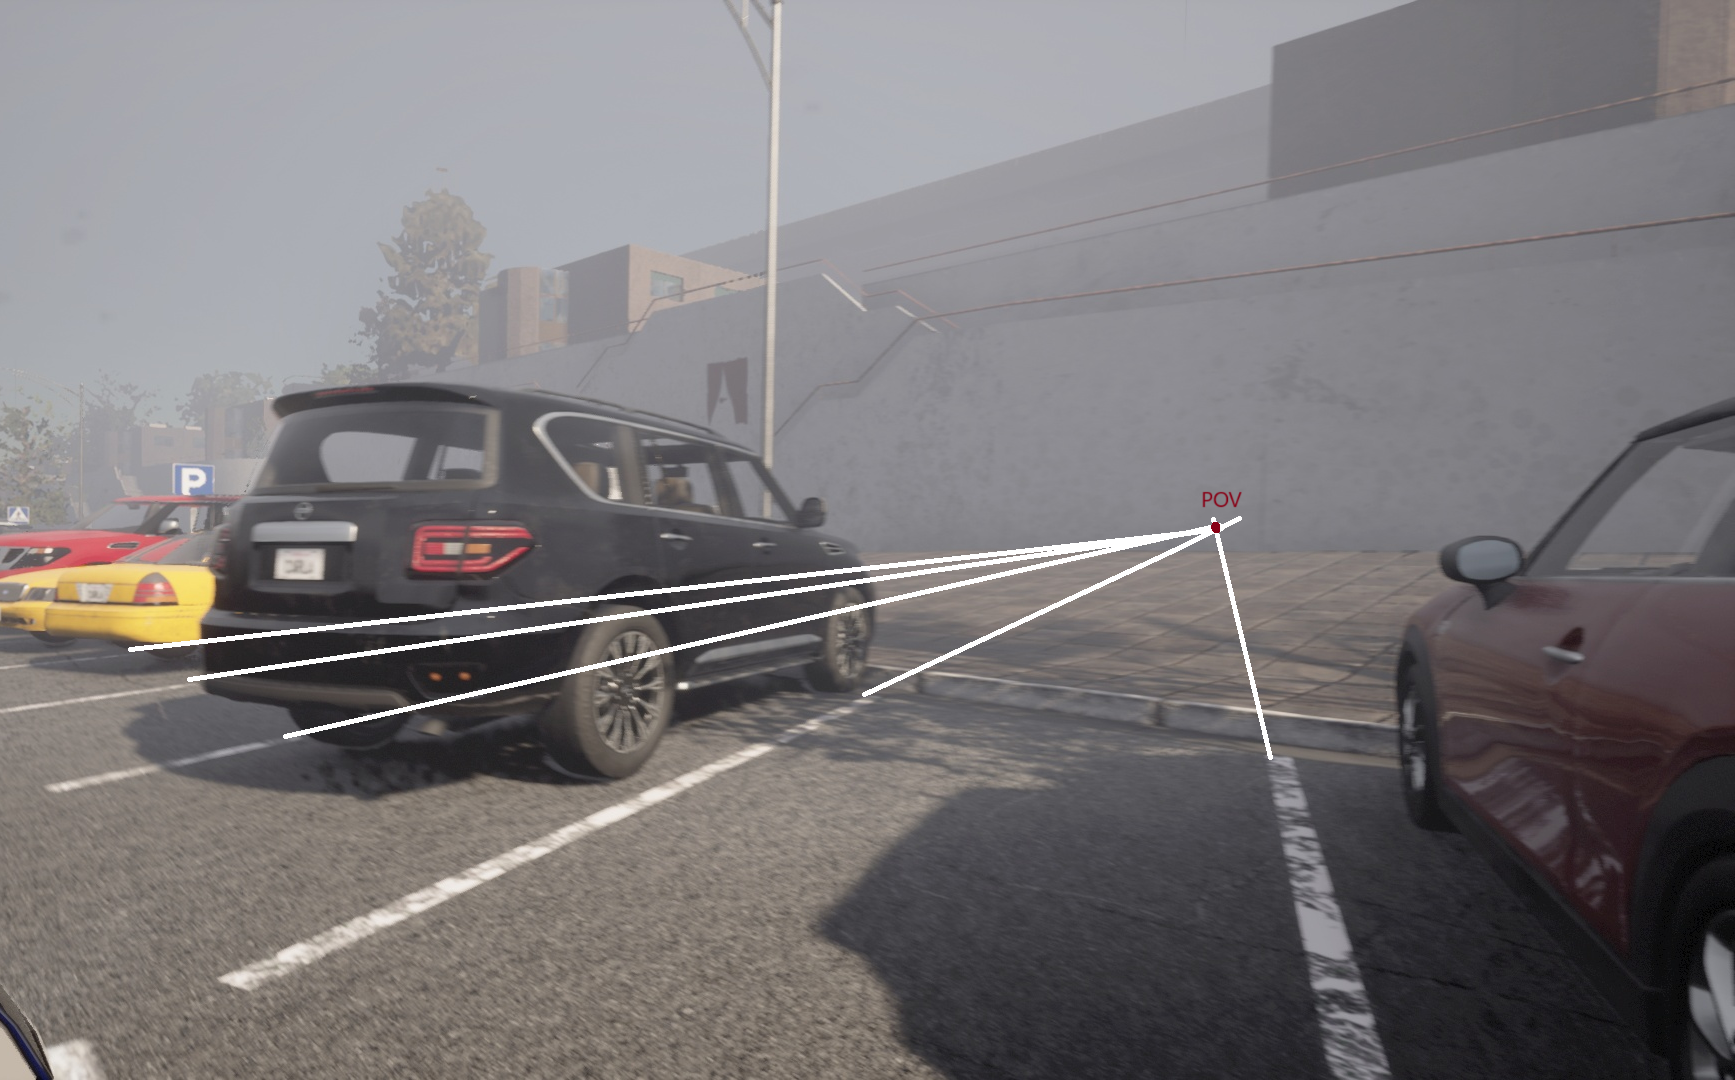
\includegraphics[width=\textwidth]{img/reticule/pov}\label {fig:pov}
        \caption{Proyección de líneas paralelas en el plano de la cámara}
    \end{subfigure}

    \label{fig:distorion}
\end{figure}

\noindent
Dado que las líneas de los cajones de estacionamiento son paralelas por su geometría, forman patrones en una retícula de paralelogramos.
Esto permite utilizar técnicas de detección de líneas para identificar los puntos de fuga y estimar la posición de la retícula de estacionamiento.

\begin{figure}[!ht]
    \centering
    \begin{subfigure}{0.8\textwidth}
        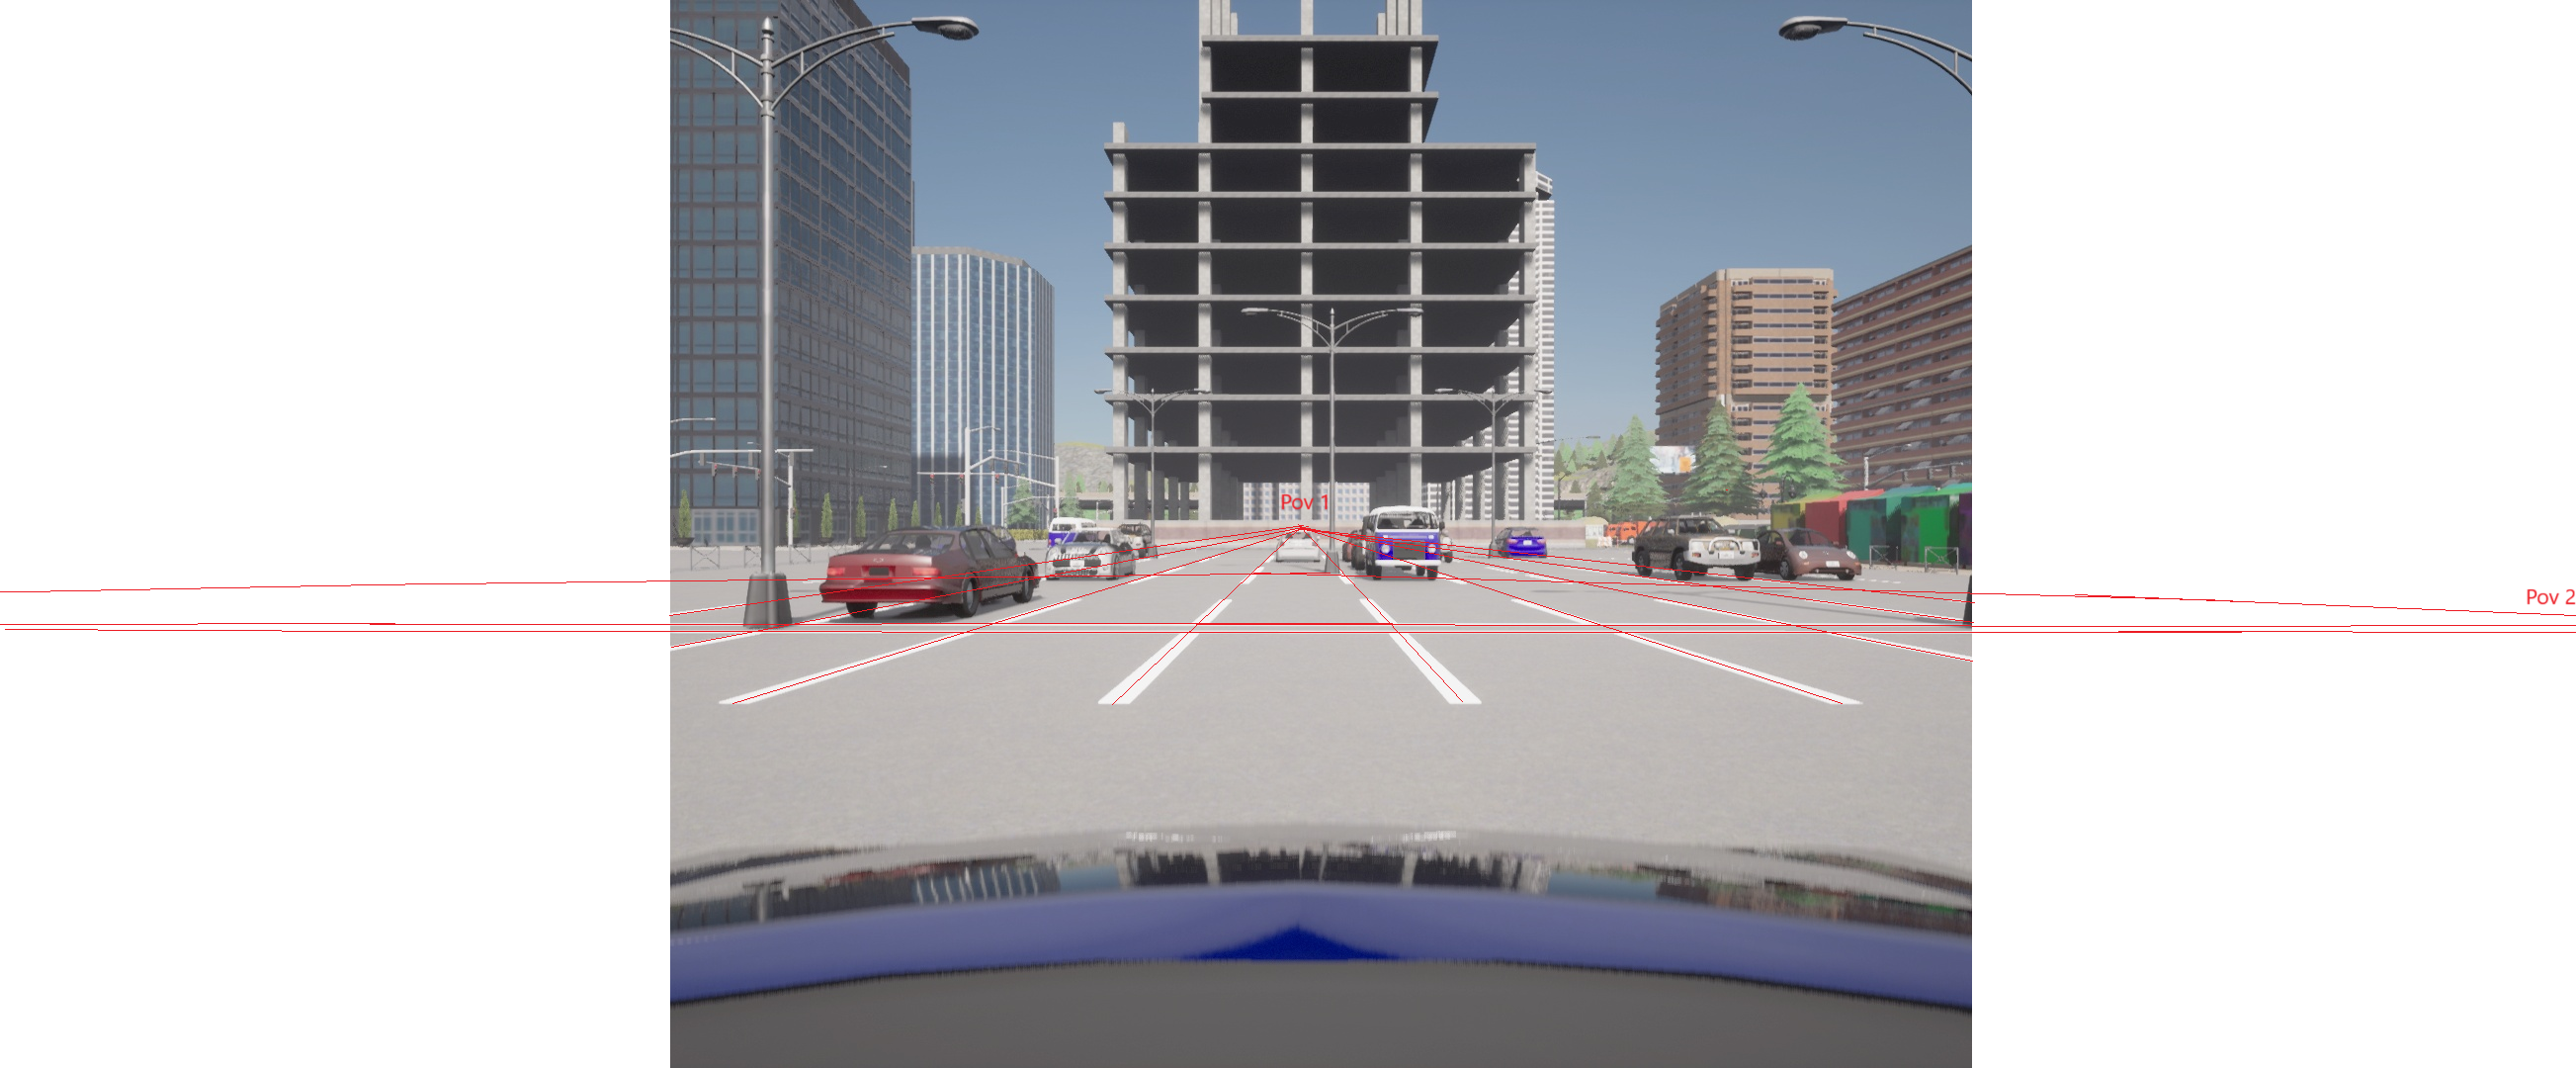
\includegraphics[width=\textwidth]{img/reticule/pov_reticule}\label {fig:pov_reticule}
    \end{subfigure}
    \begin{subfigure}{0.8\textwidth}
        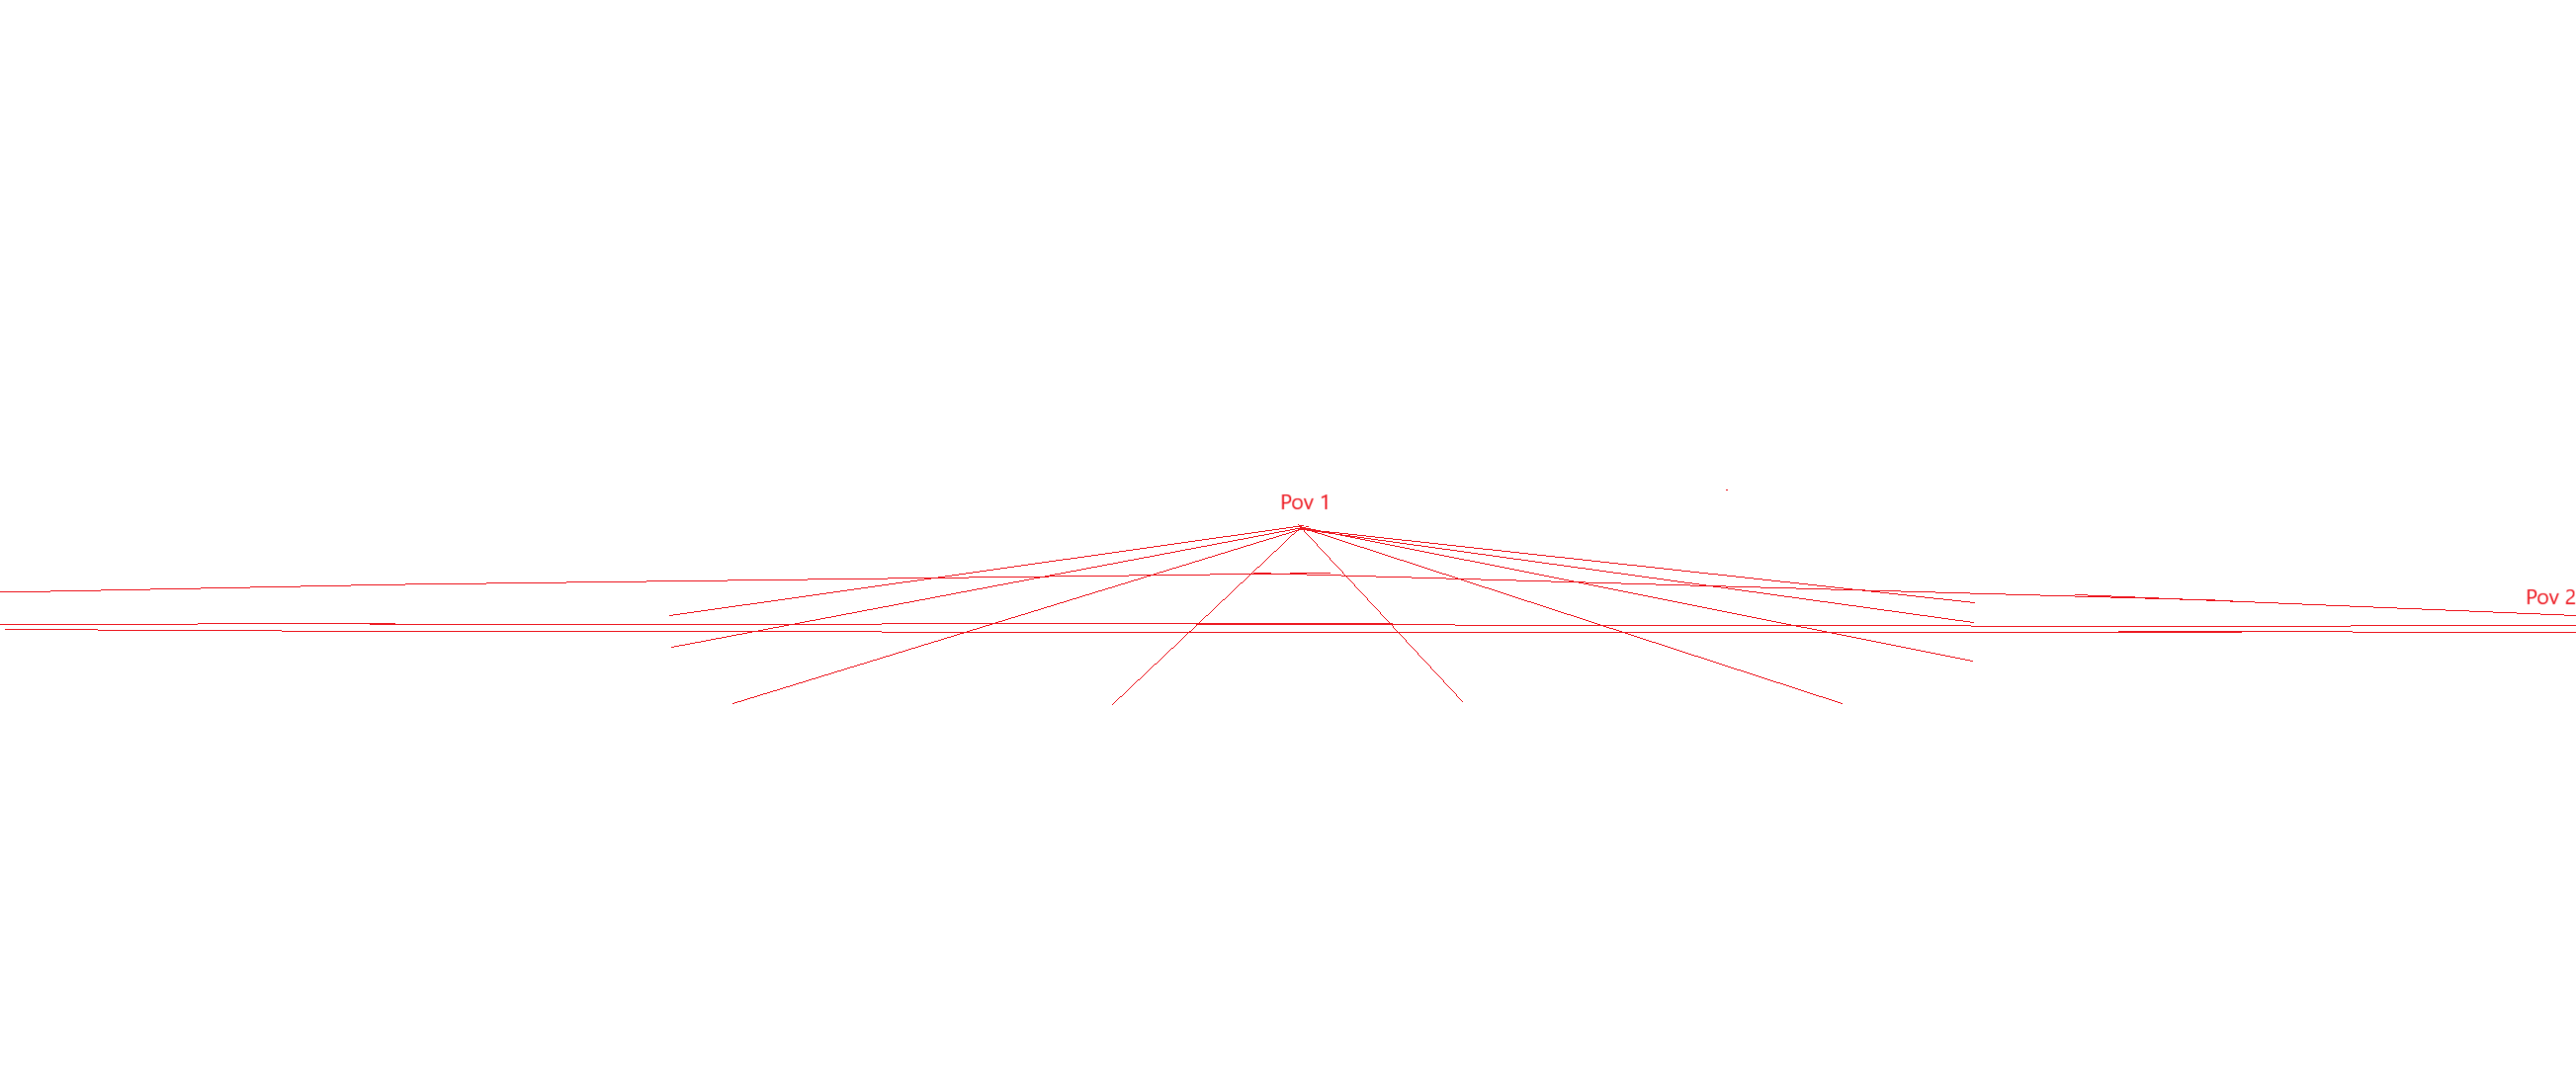
\includegraphics[width=\textwidth]{img/reticule/pov_reticule_layer}\label {fig:pov_reticule_layers}
    \end{subfigure}
    \caption{Líneas paralelas de la retícula de estacionamiento}
    \label{fig:reticule_pov}
\end{figure}

\noindent

\subsection{Detección de líneas paralelas:}

\begin{itemize}
    \item Área de interés:

    Teniendo en cuenta que la camara del vehículo se encuentra ubicada en la parte delantera a una altura conocida y en un ángulo paralelo al suelo, el área de interés de la imagen donde se encuentran las líneas de los cajones de estacionamiento quedara siempre por debajo del horizonte de la imagen.
    Por lo tanto, se puede eliminar la parte superior de la imagen para
    reducir el ruido y mejorar la detección de las líneas.
    \begin{figure}[!ht]
        \centering
        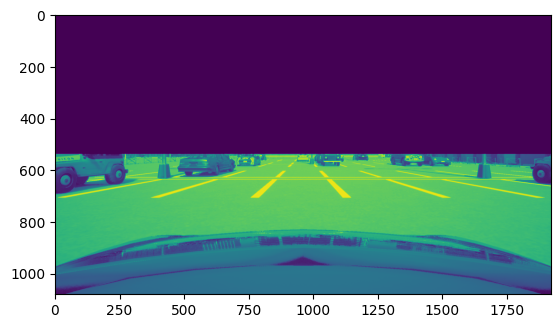
\includegraphics[width=0.6\textwidth]{img/reticule/horizont}
        \caption{Área de interés de la imagen}
        \label{fig:roi}
    \end{figure}

    \item Umbralización:

    Al área de interés de la imagen se le aplica una umbralización para realzar las líneas blancas de los cajones de estacionamiento y eliminar otros elementos no relevantes que puedan interferir en la detección.
    \begin{figure}[!ht]
        \centering
        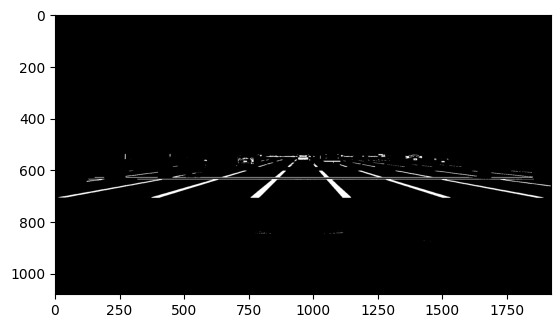
\includegraphics[width=0.6\textwidth]{img/reticule/thresholded}
        \caption{Imagen umbralizada}
        \label{fig:threshold}
    \end{figure}

    \clearpage
    \item Detección de contornos:

    Se utiliza el algoritmo de Canny para detectar los bordes de las líneas en la imagen umbralizada.
    \begin{figure}[!ht]
        \centering
        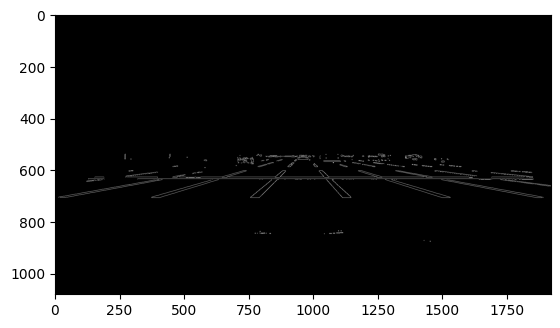
\includegraphics[width=0.6  \textwidth]{img/reticule/canny}
        \caption{Detección de bordes mediante el algoritmo de Canny}
        \label{fig:edges}
    \end{figure}

    \item Detección de líneas:

    Se aplica la transformada de Hough para detectar las coordenadas de inicio y fin de las líneas en la imagen.
    \begin{figure}[!ht]
        \begin{subfigure}{0.5\textwidth}
            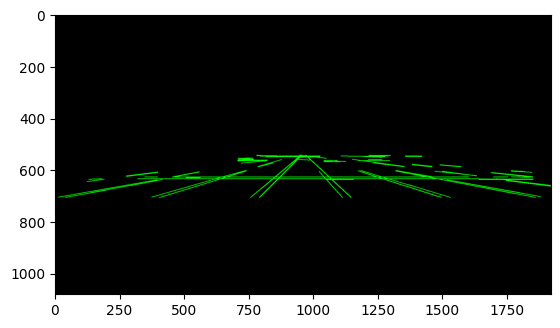
\includegraphics[width=\textwidth]{img/reticule/hough2}
            \caption{Líneas detectadas con la transformada de Hough}
            \label{fig:hough}
        \end{subfigure}
        \begin{subfigure}{0.5\textwidth}
            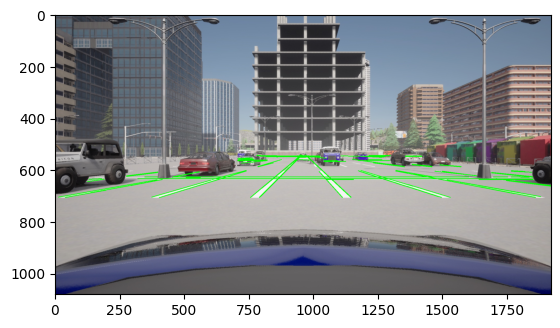
\includegraphics[width=\textwidth]{img/reticule/hough}
            \caption{Líneas detectadas en la imagen original}
            \label{fig:lines}
        \end{subfigure}
    \end{figure}

    \item Representación de las ecuaciones de las líneas:

    Una vez obtenidas las coordenadas de inicio y fin de cada línea paralela, podemos utilizar la ecuación general de la recta:
    \begin{equation}
        Ax + By + C = 0
    \end{equation}
    Esta ecuación nos permite determinar la orientación de cada línea.
    Dado que las coordenadas iniciales y finales de cada línea corresponden a los valores de $x$ y $y$, respectivamente,    estas se pueden emplear para formular un sistema de ecuaciones que describa los parámetros de la recta $[A, B, C]$.
    Dicho sistema puede representarse de manera matricial como sigue:
 \begin{equation}   
    \begin{aligned}
        \left[\begin{array}{ccc}
                  x_1 & y_1 & 1 \\
                  x_2 & y_2 & 1
        \end{array}\right]
        \begin{bmatrix}
            A \\
            B \\
            C
        \end{bmatrix}
        =
        \begin{bmatrix}
            0 \\
            0
        \end{bmatrix}
    \end{aligned}
\end{equation}

    Esta representación permite calcular de forma precisa los coeficientes de la ecuación de la recta para cada línea detectada, lo que es fundamental para analizar su orientación y posición dentro de la retícula de estacionamiento.

    \item Cálculo de ecuaciones de las líneas:

    Para calcular los coeficientes $[A, B, C]$ de las ecuaciones de las líneas detectadas, se utiliza el concepto de espacio nulo (\emph{null space}). Este enfoque se basa en el hecho de que cualquier vector en el espacio nulo de una matriz $\mathbf{M}$ satisface la ecuación
    \begin{equation}
        \mathbf{Mv} = 0
    \end{equation}

%Comentario: No has definido el vector v.
  

    Cada línea se representa mediante dos puntos $(x_1, y_1)$ y $(x_2, y_2)$. A partir de estas coordenadas homogeneas, construimos una matriz $\mathbf{M}$ de la forma:
    \[
        \mathbf{M} = \begin{bmatrix}
                x_1 & y_1 & 1 \\
                x_2 & y_2 & 1
        \end{bmatrix}
    \]
    Esta matriz define el sistema de ecuaciones que describe la recta que pasa por los puntos dados.
    El espacio nulo de $\mathbf{M}$ corresponde al conjunto de vectores $[A,B,C]$ que satisfacen
    \[
        \mathbf{M} \cdot \begin{bmatrix}
                    A \\ B \\ C
        \end{bmatrix} = \mathbf{0}.
    \]
    Se utiliza la Descomposición en Valores Singulares (SVD) para calcular este espacio nulo, ya que es una herramienta robusta y numéricamente estable.
    La SVD descompone la matriz \(M\) en tres matrices \(U\), \(S\) y \(V\), donde el espacio nulo de \(M\) se puede obtener a partir de la última columna de la matriz \(V\), que corresponde al vector singular más pequeño (el más cercano al cero).
    El vector resultante del espacio nulo se normaliza para que tenga una magnitud manejable. Esto asegura que los coeficientes \(A\), \(B\) y \(C\) sean comparables entre distintas líneas.

    \item Cálculo de intersecciones:

    Dado que ya se tendrian las ecuaciones de todas las líneas paralelas en el plano de la cámara, se pueden calcular las intersecciones de estas líneas realizando un producto cruz entre las ecuaciones homogéneas [\(A\),\(B\),\(C\)] de todos los pares de líneas.
    
    El resultado de este producto cruz es la coordenada homogénea de un punto en el espacio que corresponde a la intersección de las líneas.
    Si este punto es finito (cuando la tercera componente no es cero), se puede deshomogenizar para obtener las coordenadas cartesianas en el plano de la cámara.
    En cambio, si el punto es infinito (cuando la tercera componente muy cercana a cero), significa que las líneas son paralelas y se intersectan en el infinito.


    \item  Agrupación de intersecciones:
    %https://scikit-learn.org/stable/modules/clustering.html#hierarchical-clustering

    Analizando todos los puntos de intersecciones obtenidos que se encuentran en el plano de la cámara, se pueden agrupar para determinar donde estan
    concentrada la mayor cantidad de intersecciones. Este punto de concentración de intersecciones debe corresponder al punto de fuga principal de la retícula de estacionamiento.
    \begin{figure}[!ht]
        \centering
        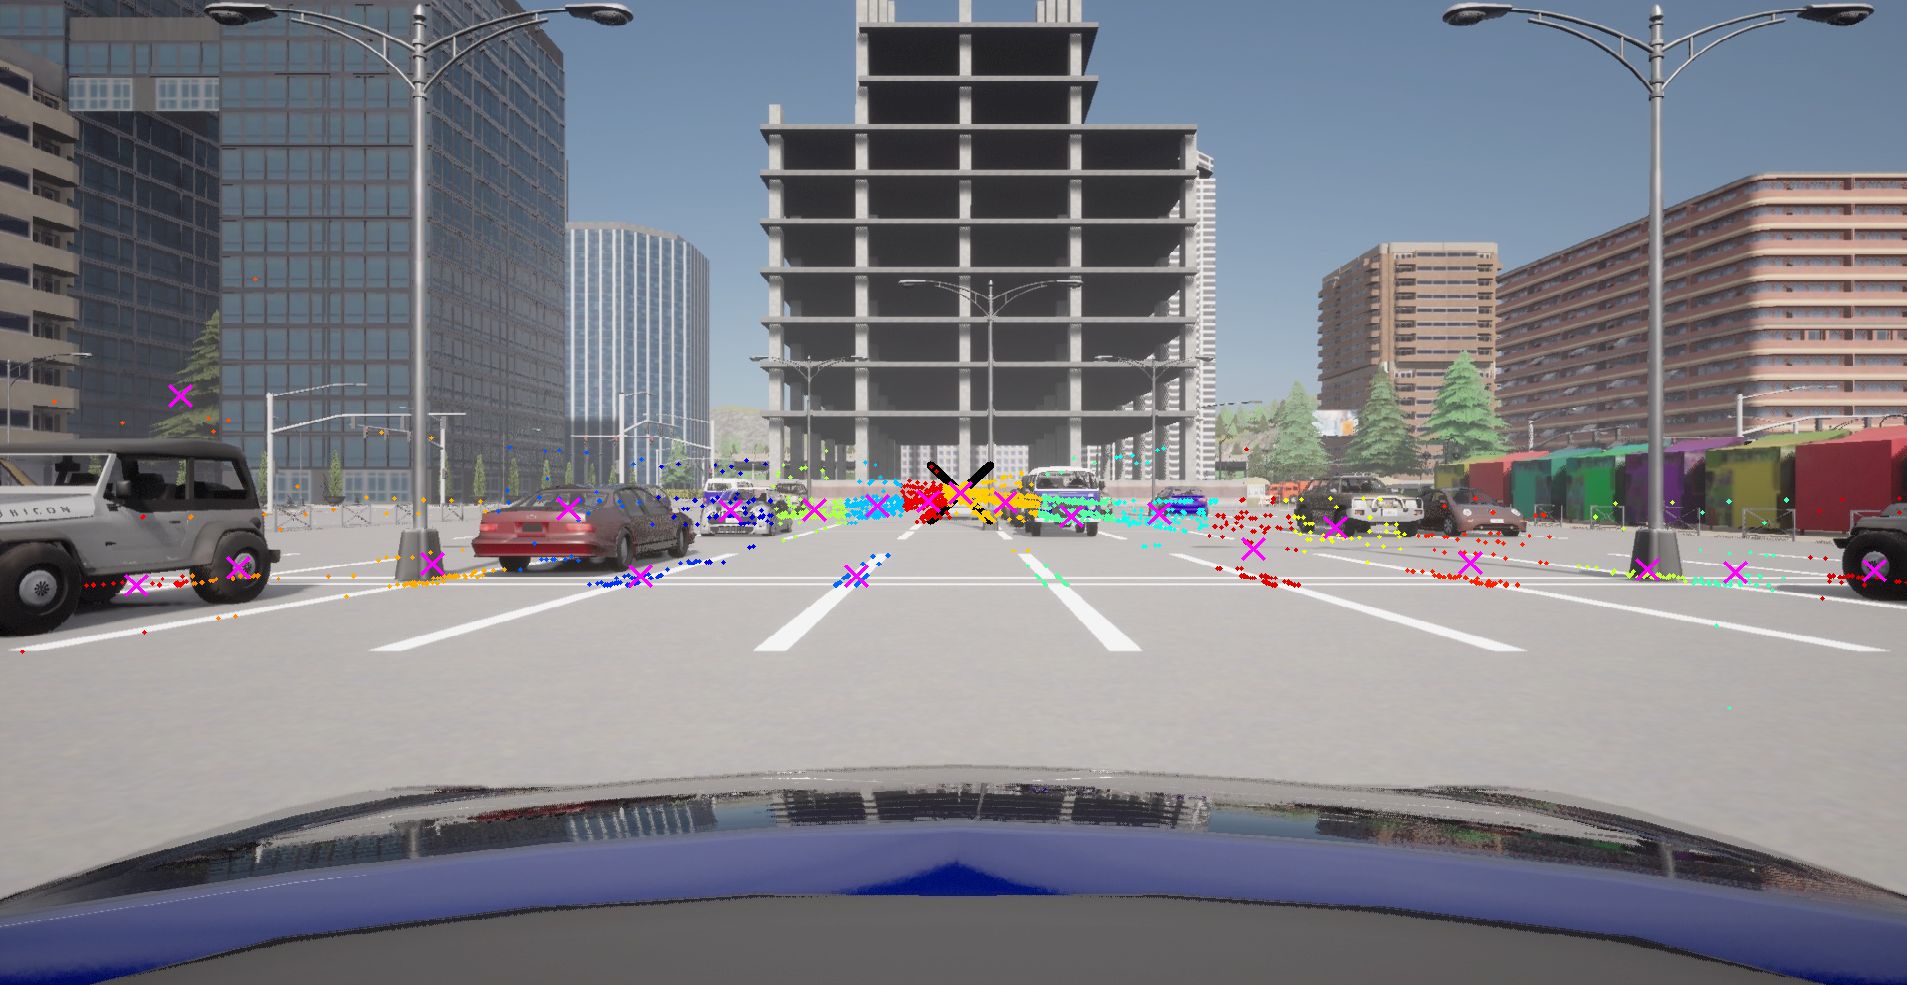
\includegraphics[width=0.8\textwidth]{img/reticule/svd-km}
        \caption{Agrupacion de intersecciones de las líneas detectadas}
        \label{fig:intersections}
    \end{figure}

    \item Selección de de puntos de fuga:
    \item Estimación de la retícula de estacionamiento:


\end{itemize}

